%% This is file `elsarticle-template-4-harv.tex',
%%
%% Copyright 2009 Elsevier Ltd
%%
%% This file is part of the 'Elsarticle Bundle'.
%% ---------------------------------------------
%%
%% It may be distributed under the conditions of the LaTeX Project Public
%% License, either version 1.2 of this license or (at your option) any
%% later version.  The latest version of this license is in
%%    http://www.latex-project.org/lppl.txt
%% and version 1.2 or later is part of all distributions of LaTeX
%% version 1999/12/01 or later.
%%
%% The list of all files belonging to the 'Elsarticle Bundle' is
%% given in the file `manifest.txt'.
%%
%% Template article for Elsevier's document class `elsarticle'
%% with harvard style bibliographic references
%%
%% $Id: elsarticle-template-4-harv.tex 167 2009-10-08 07:58:22Z rishi $
%% $URL: http://lenova.river-valley.com/svn/elsbst/trunk/elsarticle-template-4-harv.tex $
%%
\documentclass[preprint,12pt]{elsarticle}

%% Use the option review to obtain double line spacing
%% \documentclass[authoryear,preprint,review,12pt]{elsarticle}

%% Use the options 1p,twocolumn; 3p; 3p,twocolumn; 5p; or 5p,twocolumn
%% for a journal layout:
%% \documentclass[final,authoryear,1p,times]{elsarticle}
%% \documentclass[final,authoryear,1p,times,twocolumn]{elsarticle}
%% \documentclass[final,authoryear,3p,times]{elsarticle}
%% \documentclass[final,authoryear,3p,times,twocolumn]{elsarticle}
%% \documentclass[final,authoryear,5p,times]{elsarticle}
%% \documentclass[final,authoryear,5p,times,twocolumn]{elsarticle}

%% if you use PostScript figures in your article
%% use the graphics package for simple commands
%% \usepackage{graphics}
%% or use the graphicx package for more complicated commands
%% \usepackage{graphicx}
%% or use the epsfig package if you prefer to use the old commands
%% \usepackage{epsfig}

%% The amssymb package provides various useful mathematical symbols
%% The amsthm package provides extended theorem environments
%% \usepackage{amsthm}

%% The numcompress package shorten the last page in references.
%% `nodots' option removes dots from firstnames in references.
\usepackage[nodots]{numcompress}

%% The lineno packages adds line numbers. Start line numbering with
%% \begin{linenumbers}, end it with \end{linenumbers}. Or switch it on
%% for the whole article with \linenumbers after \end{frontmatter}.
%% \usepackage{lineno}
\usepackage{algorithm}
\usepackage{graphicx} 
\usepackage{url}
\usepackage[font=footnotesize]{subfig}
\usepackage{multirow}

%% natbib.sty is loaded by default. However, natbib options can be
%% provided with \biboptions{...} command. Following options are
%% valid:

%%   round  -  round parentheses are used (default)
%%   square -  square brackets are used   [option]
%%   curly  -  curly braces are used      {option}
%%   angle  -  angle brackets are used    <option>
%%   semicolon  -  multiple citations separated by semi-colon (default)
%%   colon  - same as semicolon, an earlier confusion
%%   comma  -  separated by comma
%%   authoryear - selects author-year citations (default)
%%   numbers-  selects numerical citations
%%   super  -  numerical citations as superscripts
%%   sort   -  sorts multiple citations according to order in ref. list
%%   sort&compress   -  like sort, but also compresses numerical citations
%%   compress - compresses without sorting
%%   longnamesfirst  -  makes first citation full author list
%%
%% \biboptions{longnamesfirst,comma}

% \biboptions{}

\journal{Journal of Network and Computer Applications}

\begin{document}

\begin{frontmatter}

%% Title, authors and addresses

%% use the tnoteref command within \title for footnotes;
%% use the tnotetext command for the associated footnote;
%% use the fnref command within \author or \address for footnotes;
%% use the fntext command for the associated footnote;
%% use the corref command within \author for corresponding author footnotes;
%% use the cortext command for the associated footnote;
%% use the ead command for the email address,
%% and the form \ead[url] for the home page:
%%
%% \title{Title\tnoteref{label1}}
%% \tnotetext[label1]{}
%% \author{Name\corref{cor1}\fnref{label2}}
%% \ead{email address}
%% \ead[url]{home page}
%% \fntext[label2]{}
%% \cortext[cor1]{}
%% \address{Address\fnref{label3}}
%% \fntext[label3]{}

\title{========================}

%% use optional labels to link authors explicitly to addresses:
%% \author[label1,label2]{<author name>}
%% \address[label1]{<address>}
%% \address[label2]{<address>}

\author{Po-Ching Lin\corref{cor1}}
\ead{pclin@cs.ccu.edu.tw}

\author{Yen-Chun Chiu}
\ead{5141990@gmail.com}
\address{Department of Computer Science and Information Engineering,\\ National Chung Cheng University\\ 168 University Road, Minhsiung Township, Chiayi County 62102, Taiwan \\ Tel: +886-5-2720411 ext. 33113, Fax: +886-5-2720859}

\cortext[cor1]{Corresponding author}

\begin{abstract}
Network traffic classification and characterization have been extensively applied to various purposes of network management. However, despite the high popularity of web applications, the related studies specific to their traffic are still relatively fewer than the numerous studies for generic network applications. In this work, we use \emph{application-level statistical features} to classify and characterize traffic of various web applications, such as office applications and map services. The features are quite simple, involving only the top-5 most frequent message sizes in the requests of the main connection, which is the most representative of user interactions. We manually collected packet traces from nine web applications and two browsers (Chrome and Firefox). After extracting features, we use Weka with four algorithms to evaluate the accuracy, i.e., NBtree, Random Forest, J48graft and Naive Bayes. The experiment results show the accuracy can be up to 93.89\% with random forest. Furthermore, this mechanism allows early classification with only the first 30 messages in the main connection and the accuracy can also achieve up to 93.89\% with random forest. In addition, we collected the traffic from multiple users to evaluate classification, and the result shows that the features can also classify such traffic effectively.
\end{abstract}

\begin{keyword}
traffic classification and characterization \sep web applications \sep application-level features
%% keywords here, in the form: keyword \sep keyword

%% MSC codes here, in the form: \MSC code \sep code
%% or \MSC[2008] code \sep code (2000 is the default)

\end{keyword}

\end{frontmatter}

% \linenumbers

%% main text
\section{Introduction}
\label{sec:intro}

A variety of web applications have been increasing rapidly in recent years, such as webmail services, web-based online games, file sharing, video streaming. World wide web has become a popular platform for developing various network applications since users can access the applications all from a browser instead of installing individual applications. This trend is expected to persist with the popularity of cloud computing and network protocols such as WebSocket, which all enrich the features of web applications.   
	
Just like non-web network applications, the traffic from web applications should be classified for various purposes, including policy-based control, quality-of-service (QoS), auditing and security management. In this work, we intend to \emph{differentiate the traffic from various web applications and identify the user interactions in the applications}. However, almost all web applications run on HTTP(S) related ports, i.e., TCP ports 80 and 443, and their packet payloads are usually encrypted, so it is usually impossible to classify web applications according to port numbers and deep packet inspection on packet payloads \cite{ASO08,PIO13}. Since classification by port numbers and packet payloads is infeasible for web applications, machine learning approaches to classification based on statistical features such as number of packets in a flow, byte frequency, packet size and packet inter-arrival time are promising. The approaches have been intensively studied in prior research for generic network applications \cite{COS04}.

We pointed out such statistical features may be unreliable in a prior study \cite{TFT14} because they are subject to various network conditions such as network congestion (which affects packet inter-arrival time), maximum transmission unit (MTU) in different link-layer networks (which affects packet sizes and number of packets in a flow), packet loss and retransmission (which affect number of packets in a flow), etc. Moreover, different user interactions even in a single web application may generate network traffic of diverse characteristics. For example, the traffic characteristics from typing a keyword to be searched and from map browsing in a map application are obviously different. Google drive not only supplies a platform for users to edit a document, but also to up/download files. In other words, the traffic characteristics that a web application exhibits will vary with the composing user interactions in each run. Thus, the features in classification should be carefully selected to not depend on the composition in a particular run.
   
According to the above arguments, this work also uses statistical features from application messages in web applications like our previous work \cite{TFT14}, which has several limitations in practice. (1) It is unclear whether or not all the connections observed during a user interaction should be attributed to that interaction. Because it is infeasible to observe the messages carried in encrypted connections, we use a developer tool such as Firebug (\url{getfirebug.com}) on the browser to observe the content in each connection and recognize the main connection responsible for a user interaction, e.g., typing a keyword to be searched or downloading a video clip. Thus, the features derived from the main connection can better reflect the user interaction than those from the other minor connections such as those for downloading advertisements. (2) It is difficult to locate the beginning and the end of a user interaction in a connection because the packets related to more than one interaction may be carried over a single connection. Thus, identifying the packets belonging to a user interaction for feature extraction may be imprecise in classification. In this work, we extract the features from the main function, whose beginning and end are rather clear. (3) The features in the prior work are extracted from the entire set of packets during a user interaction, so the classification cannot make a decision until all the packets of an interaction have been observed. The limitation makes it difficult to deploy the classification in the prior work for access control, which needs to determine the web application as early as possible when the traffic is passing through a gateway. In this work, we also evaluate the classification accuracy based on the feature from the first few messages in a main connection. 

This work evaluates the accuracy of traffic classification and the characterization for web applications. The main contributions of this paper are as follows:

\begin{enumerate}
\item 
We characterize the traffic from typical web applications, even if the messages are encrypted in the packet payloads, with the help of the developer tool affiliated to a browser.
\item
We identify the main connection to classify web applications. The features extracted from the main connection can better reflect the user interaction than those from the other connections.  
\item
This mechanism allows early classification with only the first 30 messages in a main connection and the accuracy can be up to 93.89\% with random forest. 

\end{enumerate}

The remainder of this work is organized as follows. Section~\ref{sec:background} reviews related work. Section~\ref{sec:method} describes the inference methodology, and emphasizes the main differences between the methods in this work and previous ones. Section~\ref{sec:evaluation} describes the data sets for evaluation and validations. Finally, We conclude this work and present future work in Section~\ref{sec:conclusion}.

\section{Background and Related Work}
\label{sec:background}
Prior studies have proposed many traffic classification approaches, including port-based \cite{TTC}, payload-based, flow-based and host-based techniques \cite{TCI13}. We review the last three methods and the studies about the web traffic classification in this chapter.    


\subsection{Payload-based classification}
\label{sec:payload}
Payload-based traffic classification means determining the application of the traffic according to packet payloads. It usually looks for application patterns represented in fixed strings or regular expressions. A typical example is nDPI (\url{www.ntop.org/products/deep-packet-inspection/ndpi}). Hullar et al. \cite{EMF14} presented a method to analyze only the first few bytes of the first (or first few) packet(s) of each flow for early protocol identification. The method has the advantage of accurate classification and easy development, but may lose its effectiveness if the payloads are encrypted. Moreover, maintaining the patterns of numerous applications is also a non-trivial effort as the applications usually keep evolving.

%OpenDPI \cite{ODA12} is an open-source classifier derived from early versions of PACE \cite{PACE}, and it learns the five-tuple information, which includes a source IP address/port number, destination IP address/port number and the protocol in use, of the data flow by inspecting the payload of the control flow. The method implements its own connection tracking functionality. After receiving the packets, OpenDPI calls the connection tracking function, and then calls the plugins one by one. All plugins are called for each function, so it may found various protocol be matched, however, the one at the highest level is returned. Nevertheless, the string-based matching has the problem of limited expressivity, so the regular expression matching was proposed.

%There is the typical example of the regular expression matching \cite{l7-filter}, which is a classifier for Linux's Netfilter. The technique can classify packets as HTTP, FTP, Bittorrent, and so on. L7-filter provides a set of pattern definition files and wouldn't to run a regular expression matcher on every packet, so it can save much more time and resource than Open-DPI.

\subsection{Flow-based classification}
\label{sec:flow}
Another expanding set of classification techniques are based on machine learning with statistical features of network traffic. The studies in \cite{EAI06, ATC13} classify the behavior of an application by the size and the direction of the first few packets of a TCP connection. Bernaille et al. \cite{EAI06} defines the behavior of an application as the size and direction of the first four packets it exchanges over a TCP connection. An et al. \cite{ATC13} uses the first five packets and converts the flow into a vector. The paper shows the possibility of classifying traffic using the payload size distribution of the packets; nevertheless, this method classifies all application traffic, except HTTP.

Some studies \cite{AIS14, CMF04, COC12} extract the features from a complete flow. Common features are port numbers, average segment size, internal time of packets, and so on. \cite{AIS14} uses a Fast Correlation-Based Filter (FCBF) to choose the essential feature, which can reduce the processing time. 

Furthermore, some studies \cite{FPN13, RTC10, AIS14, ASA09, FTC09} used clustering techniques in machine learning to classify traffic. \cite{FPN13, RTC10} are based on Naive Bayes algorithm, a supervised machine learning algorithm based on Baysian theory. Artificial Immune System (AIS) algorithm is proven to be very versatile and low sensitivity to input parameters, so \cite{AIS14} used it as their base. The study implemented the features as hyper spheres within an 11-dimensional space, and if an example vector falls within the distance of the hyper sphere, then the example is classified to the same class as the feature belong to. The rest of studies are based on k-Nearest Neighbor (KNN) estimator \cite{ASA09} and on support vector machine (SVM) \cite{FTC09}. Machine-learning-based classification can automatically build a model from training data and reduce much artificial input; however, the classification will decrease because they only collect and classify traffic in a limited range. The limitation is a challenge. It is difficult to identify all protocols by using only a machine learning model because most models are binary classification, which means one model just can classify one protocol.

  
\subsection{Fine-grained classification}
\label{sec:grained}
The main idea behind fine-grained traffic classification is how to categorize application traffic into different traffic groups, and it has some advantages to improve the network security and the QoS management. There are some instances below:

S. Valenti et al. presented \cite{FBC11}, which use the Abacus behavioral classification engine and SVM to categorize the P2P traffic. They apply the traces of the six P2P applications, ranging from file-sharing to VoIP and live-streaming services, such as SopCast, Skype and BitTorrent. The research use Abacus classifier by only relying on the count of packets and bytes peers exchange during fixed-length time-windows, but the accuracy would be decreased when the vantage points moves from the edge.

In \cite{TFT11}, the authors select P2P applications for verification since the various behavior can strongly represents the complexity of Internet applications. P2P applications provide many functions: web browsing, searching, downloading, messenger and commercial advertisement. This paper uses Fileguri and BitTorrent to generate the flows, and creates the signatures by fine-grained classifier and LASER. They collected 450Gbytes from their campus network, then transform each packet into a vector, and exploited Jaccard for clustering.

\
\begin{table}[H]
\centering
\caption{Pros and cons of each classification.}
\begin{tabular}{|l|p{3.5cm}|p{3.5cm}|p{3.5cm}|}
\hline Classification & Features & Pros and Cons & Used in studies \\
\hline
\hline Port-based & well-known port numbers & simply and fast but can't be used in the tunnelling traffic & \cite{TTC}\\
\hline Payload-based &  string-based matching, regular expression matching and IP protocol & accurate classification capability and easy development but slow and can't be used in encrypted traffic & \cite{nDPI} , {l7-filter} \\
\hline flow-based & packet size, packet inter-arrival time, flow duration, packet numbers,etc. & can detect the class of yet unknown applications but cannot deal with multiple transport transport protocols simultaneously & \cite{EAI06}, \cite{ATC13}, \cite{AIS14}, \cite{CMF04}, \cite{COC12}, \cite{FPN13, RTC10, AIS14, ASA09, FTC09} \\
\hline 
\end{tabular}
\label{table:pros-cons}
\end{table}


\subsection{Web traffic classification}
\label{sec:web}

In recent years, some studies have taken steps toward classifying web traffic classifications \cite{TFT14, OTP11, DHC11, MAM13}. In \cite{MAM13}, P. Casas et al. designed a classifier named Mini-IPC. The technique uses only the IP addresses of the servers hosting the corresponding content to classify HTTP flows. Since multiple different services may be associated to the same IP address, the authors use a random selection approach to solve the issue. Lin et al. classified the HTTP traffic using libnids (\url{libnids.sourceforge.net}) to reassemble the message and computing the average and the standard deviation of the request/response lengths as the features for the classifier. Different from some previous studies, the features are independent of the network condition under the application layer. The accuracy can reach up to 92\%.



%In \cite{DHC11}, R.Archibald et al. investigate representatives of classes of web applications, namely Facebook, Gmail, Youtube, which apply HTTP as their communication protocol. They classify the applications based on any segment of the bidirectional flow, and derive the packet sizes and inter-arrival times from the flow as their features. This study even applies simple statistical and spectral analysis to distinguish the traffics. Finally, they show that despite the noises of packet padding and altering the inter-packet delay, using the classifier also can maintain a classification rate of up to 60\% .



\subsection{Web traffic characterization}
\label{sec:web_type}
Web 2.0 features that users can interact and cooperate with each other in a social media dialogue as creators of user-generated content in a virtual community, and Ajax application is one of the client-side technologies used in Web 2.0 development. Ajax can actively fetch data before a user's request. Because the increasingly development based on Ajax, characterizing the applications is also increasingly important. M. Lee et al. presented a tool \cite{AAM10} to characterize the traffic derived from Google maps and mail. The technique can automatically interact with Ajax-powered cloud services, and utilizes a traffic shaper to control network latencies and bandwidth to distinguish the traffic. Some studies are dedicated to characterizing Web 2.0 applications \cite{MTC09, COH08, WTM09}. S. Veres et al. presented a method that focuses on analyzing and characterizing traffic up to the transport layer, and uses average packet rate, bandwidth, inter-arrival time and packet size for the characterization.

\section{Method of Web Traffic Classification}
\label{sec:method}
Precise traffic classification relies on a clear understanding of web traffic. However, as application protocols and development techniques of web applications keep evolving (particularly, the HTTP/2 protocol \cite{HTTP2} and new development techniques such as Ajax and node.js in recent years), the traffic characterization of web applications in prior studies may not reflect the state-of-the-art. Therefore, it is necessary to re-examine the traffic characteristics from typical web applications, and find out effective features for precise classification. Typical features in traffic characterization usually include application payloads, packet size, connection length and duration, packet inter-arrival time, and so on. We argued in \cite{TFT14} that the features may be unstable due to the variations of Internet traffic. In this work, we focus primarily on the application-level features that are not subject to the conditions in underlying networks. We study the traffic characteristics in popular web applications, including office applications (Google document), maps (Google maps), file sharing (Google drive and dropbox), video streaming (Youtube, Dailymotion, Tudou), and online games (Tetris battle and Dungeon Rampage on Facebook), in terms of the features on various browsers. We then extract the features from the main connection described in next section, so we do not need to compute the average and the standard deviation of the request/response lengths like \cite{TFT14}. 

\subsection{Data collection}
\label{sec:collect}

A web application usually involves highly user interactions between the browser and the web server. Developers often use techniques such as Ajax to improve user experiences, e.g., by actively pushing web content to the browser before the user requests it. Moreover, new application protocols, particularly SPDY (\url{www.chromium.org/spdy}) primarily developed at Google and HTTP/2 based on SPDY, support features to reduce the latency of loading web pages for efficient web browsing. Major browsers such as IE, Firefox and Chrome have supported SPDY and HTTP/2, and most of them have enabled the support by default at the time of this thesis writing. The web traffic from the Google services covered in this work is all sent over SPDY. However, the traffic  from the other web applications (see Table~\ref{table:scenario_app}) also use SPDY, except that from Facebook, Dailymotion and Tudou. Thus, the traffic studied in this work reflect the latest status in the development of web applications.  

Since a browser may keep prior web content in a local cache to speed up web browsing, we use the guest mode of a browser (in which the web content in prior browsing will not be preserved) when interacting with a web application to ensure a complete set of packets during the interaction can be collected. We browse only a specific web application at a time to ensure the web traffic is all from that application, and use Wireshark (\url{www.wireshark.org}) to collect the packets. 

In this work, we consider several typical scenarios of using web applications, and capture the web traffic from them. This work covers totally five types of 9 web applications, as listed in Table~\ref{table:scenario_app}. We implore users to operate each web application on either Chrome or Firefox in the scenarios described in this table. A user is requested to interact with the applications for a period from one to two minutes as usual. We do not use Internet Explorer for several reasons. First, the browser is not supported on many operating systems, e.g., Mac OS and Android \cite{IBR}. Second, the usage of IE is reported to be dropped to only 7.1\% \cite{BS}. Third, Windows 10 no longer supports IE. 



\begin{table}[ht]
\centering
\caption{The scenario of each web application.}
\begin{tabular}{|l|l|p{0.2\linewidth}|p{0.45\linewidth}|}
\hline no. &type &application &scenario \\
\hline
\hline 1 &Document &Googledoc & arbitrarily typing and editing\\
\hline 2 &Map  &Googlemap & typing a location name, arbitrarily browsing the map and zooming-in and zooming-out\\
\hline 3-5 &Video  & Youtube/ Tudou/ Dailymotion & typing a video name and arbitrarily moving to a specific time position during watching\\
\hline 6-7 &File transfer & Google drive/ Dropbox & up/downloading \\
\hline 8-9 &Gaming &Facebook : Tetris Battle/ Dungeon Rampage & arbitrary operation\\
\hline 
\end{tabular}
\label{table:scenario_app}
\end{table}



\subsubsection{Extract statistical signature}
A web application server may offer two or more services, so identifying the application based solely on the server's IP address is unreliable. For example, Google offers all its services on the same back-end server infrastructure (e.g., Google document and Google map can be provided by the same IP address 74.125.23.102 in our observation.), so users can reuse existing TCP connections to Google servers to access the other services \cite{TNW08}. Thus, classification with statistical features to distinguish the traffic from various web applications is necessary. 

There are several requirements for the training packet traces to acquire precise application-level statistical features:
\begin{enumerate}
\item 
The collected packet traces must be generated only from the targeted web application. We set the filter of Wireshark to capture the packets from or to port 80 and 443, and ask the user runs only a web application on the browser for every time of packet collection.
\item
The packets in the beginning of connections should be preserved for TCP state tracking, which is necessary for packet reassembly to recover the application-level features.
\item
The collected traffic should be sufficient and diverse because it may affect the accuracy and reliability. The collected traffic must contain the packet traces from the user interactions from the targeted web application. Moreover, we performed various interactions on a same web application for every collection to ensure the diversity of packet traces. For example, we changed the frequency of typing extremely every time when we collected the traffic from Google document.
\end{enumerate}

We set the target IP address and ports and follow the scenarios listed in Table~~\ref{table:scenario_app} to run the web applications when collecting the training packet traces. The quantity of collected traffic is important to reflect practical user behavior precisely. We take advantage of this to observe whether diverse user behaviors will impact on the classification or the characterization. Not only the user interactions, but also the environment will influence the results. For example, some browsers support the SPDY protocol, but Mozilla Firefox did not until 2011. The difference will influence the patterns of some flows when the packets are carried over different protocols.

After collecting a new set of packet traces for a web application in the training set, we find the main connection by using the developer tool affiliated to the browser (e.g., Firebug on Firefox), which allows developers to view information about the transmitted messages. Hence we confirm which connection is the most representative of the user interactions by referring to the parameters in the HTTP messages summarized in Table~\ref{table:judge_main}. Nevertheless, many simultaneous connections may load web information in Table~\ref{table:content_other} to provide smooth user experiences, so we choose the longest one as the main connection. The only exception is the main connection for Tetris Battle, which transfers the elements related to the game platform instead of the game interactions. Thus, our mechanism takes advantage of this property to decide the main connection when a set of packet traces are analyzed. We can effectively segregate the noise, such as embedded advertising, with the method. This work uses the \texttt{libnids} library (\url{libnids.sourceforge.net}), which offers IP defragmentation, TCP stream reassembly and TCP port scan detection, to reconstruct the request-response streams of all the connections. The tool needs to track the states of TCP connections, so the beginning time of packet capturing is crucial to ensure important state transitions, e.g., 3-way handshaking, are not missing. We extract the source/destination IP addresses and source/destination ports to recognize each flow.




\begin{table}[ht]
\centering
\caption{The judgment of the main connection.}
\label{table:judge_main}
\begin{tabular}{|l|l|l|}
\hline
              & Referred parameter                                                        & \multicolumn{1}{c|}{Judgment}                                                                                                                                                                                                                                                                                                            \\ \hline \hline
Document      & bundles                                                                    & \begin{tabular}[c]{@{}l@{}}contain some arrays to store the characters we typed\end{tabular}                                                                                                                                                                                                                                              \\ \hline
Map           & content-type                                                               & \begin{tabular}[c]{@{}l@{}}(1)image/png : comparing whether the preview picture\\     and the map showed on the website are the\\     same or not\\ (2)application/vnd.google.octet-stream-\\     compressible;charset=x-user-defined : this \\     message continuously appear as we \\     arbitrarily send actions to the map\end{tabular} \\ \hline
Video         & content-type                                                               & For example, audio/mp4, video/webm and video/f4v.                                                                                                                                                                                                                                                                                           \\ \hline
File transfer & \begin{tabular}[c]{@{}l@{}}content-disposition\\ content-type\end{tabular} & \begin{tabular}[c]{@{}l@{}}(1)checking the filename in the content-\\     disposition match with the file we \\    transfer \\ (2)comparing the content-type match with the\\     file we transfer\end{tabular}                                                                                                                     \\ \hline
Game          & content-type                                                               & \begin{tabular}[c]{@{}l@{}}the content-type is application/x-shockwave-flash\\ game applications always use .swf to transfer files\end{tabular}                                                                                                                                                                                              \\ \hline
\end{tabular}
\end{table}

\begin{table}[ht]
\centering
\caption{The contents of other connections }
\label{table:content_other}
\begin{tabular}{|l|l|l|}
\hline
\multicolumn{1}{|c|}{Label}    & \multicolumn{1}{c|}{Web application} & \multicolumn{1}{c|}{Content-Type}                                                                                                         \\ \hline \hline
Document                       & Google doc                           & \begin{tabular}[c]{@{}l@{}}application/json, text/html, text/javascript, \\ font/woff, image/png, image/gif, etc.\end{tabular}            \\ \hline
Map                            & Google map                           & \begin{tabular}[c]{@{}l@{}}application/json, text/javascript, image/gif,\\ image/png, etc.\end{tabular}                                   \\ \hline
\multirow{2}{*}{Game}          & Dungeon Rampage                      & \begin{tabular}[c]{@{}l@{}}text/html, application/x-javascript, image/png, \\ application/x-shockwave-flash, etc.\end{tabular}            \\ \cline{2-3} 
                               & Tetris Battle                        & \begin{tabular}[c]{@{}l@{}}image/gif, image/png, application/xml,\\ application/x-shockwave-flash, audio/mpeg, etc.\end{tabular}          \\ \hline
\multirow{2}{*}{File Transfer} & Google Drive                         & \begin{tabular}[c]{@{}l@{}}text/javascript, application/json, text/css, \\ text/html, image/gif, etc.\end{tabular}                        \\ \cline{2-3} 
                               & Dropbox                              & \begin{tabular}[c]{@{}l@{}}application/x-javascript, image/gif, image/png,\\  application/octet-stream, text/css, etc.\end{tabular}       \\ \hline
\multirow{3}{*}{Video Stream}  & Youtube                              & \begin{tabular}[c]{@{}l@{}}audio/mp4, video/mp4, text/javascript, text/css,\\ application/x-shockwave-flash, image/gif, etc.\end{tabular} \\ \cline{2-3} 
                               & Dailymotion                          & \begin{tabular}[c]{@{}l@{}}application/x-shockwave-flash, text/css, \\ text/xml, image/jpeg, application/x-javascript, etc.\end{tabular}  \\ \cline{2-3} 
                               & Tudou                                & \begin{tabular}[c]{@{}l@{}}application/x-shockwave-flash, image/jpeg,\\ application/octet-stream, text/xml, image/gif, etc.\end{tabular}  \\ \hline
\end{tabular}
\end{table}

\subsubsection{Feature definition} 
We assume that $f_m$ is the main connection when a user interacts with a certain web application, and extract all $n$ messages to be analyzed (after processed by \texttt{libnids}). Let $s_i$ be the $i$-th message size in the request connection, where $i=1\ldots n$. We do not adopt the features in the bi-direction because including the features from the responses will introduce more ambiguity between some web applications. For example, the features generated from file download applications are sometimes similar to those from games and maps, and will decrease accuracy by 6\% according to our preliminary experiment (not shown in Chapter 4). This work counts the occurrence frequency of each message size, and takes the top five frequent sizes to be represented as a vector $v_i$ for every main connection.

Table~\ref{table:feature_doc} presents an example, in which we arbitrarily typed in a Google document on Chrome for around two minutes. Thus, the feature to characterize this interaction is (38, 34, 220, 224, 116). However, the number of different message sizes may be less than five to form a five-tuple vector. We take two ways to solve this problem. Table~\ref{table:fill_max} is generated by watching a video clip on Dailymotion with Chrome. It describes that there is a vacancy within the vector. We can fill up the missing tuple with the mode (i.e, the most common value) of the other message sizes \cite{DM}, and the vector becomes (636, 665, 658, 589, 636). Table~\ref{table:fill_same} is generated by downloading a file from Dropbox on Firefox. The occurrence time of all message sizes are the same in this table. We choose the first one to fill up the vacancies, and the vector is (753, 202, 162, 753, 753). The message sizes mentioned in these three tables are sorted by the occurrence times in the decreasing order. The features are stable and the testing results are showed in Section~\ref{sec:result}.

\
\begin{table}[H]
\centering
\caption{A feature of editing by Google document.}
\begin{tabular}{|l|c|c|c|c|c|c|c|c|}
\hline  & $s_1$ & $s_2$ & $s_3$ & $s_4$ & $s_5$ & $s_6$ & ... & $s_n$\\
\hline
\hline Message size (bytes) & 38 & 34 & 220 & 224 & 116 & 199 & ... & $m_n$ \\
\hline Count & 177 & 177 & 37 & 27 & 13 & 12 & ... & $c_n$\\
\hline 
\multicolumn{9}{l}{The vector is (38, 34, 220, 224, 116).}\\
\end{tabular}
\label{table:feature_doc}
\end{table}

\
\begin{table}[H]
\centering
\caption{A feature of downloading by Dailymotion.}
\begin{tabular}{|l|c|c|c|c|c|}
\hline  & $s_1$ & $s_2$ & $s_3$ & $s_4$ & $s_5$ \\
\hline
\hline Message size (bytes) & 636 & 665 & 658 & 589 &\\
\hline Count & 4 & 3 & 2 & 1 &\\
\hline
\multicolumn{6}{l}{The vector is (636, 665, 658, 589, 636).}\\ 
\end{tabular}
\label{table:fill_max}
\end{table}

\
\begin{table}[H]
\centering
\caption{A feature of downloading by Dropbox.}
\begin{tabular}{|l|c|c|c|c|c|}

\hline  & $s_1$ & $s_2$ & $s_3$ & $s_4$ & $s_5$ \\
\hline
\hline Message size (bytes) & 753 & 202 & 162 &  &\\
\hline Count & 1 & 1 & 1 &  &\\
\hline
\multicolumn{6}{l}{The vector is (753, 202, 172, 753, 753).}\\ 
\end{tabular}
\label{table:fill_same}
\end{table}


\subsection{System Workflow}
\label{sec:system}
Figure~\ref{Fig.system} illustrates the workflow of the classification process. A user may use either Mozilla Firefox or Google Chrome to run a web application as mentioned above. Simultaneously, the capture filter for the web application traffic is set to port 80 and 443 on the PC. The developer tool and Wireshark is employed to find the main connection that reflects user interactions most. Next, \texttt{libnids} will reassemble the captured packets to extract application-level messages. In the last step, these features extracted from the messages are fed into Weka (\url{http://www.cs.waikato.ac.nz/ml/weka}) for traffic classification with four machine learning methods: NBTree, Random Forest, J48graft and Naive Bayes.


\begin{figure}[H]
\begin{center} 
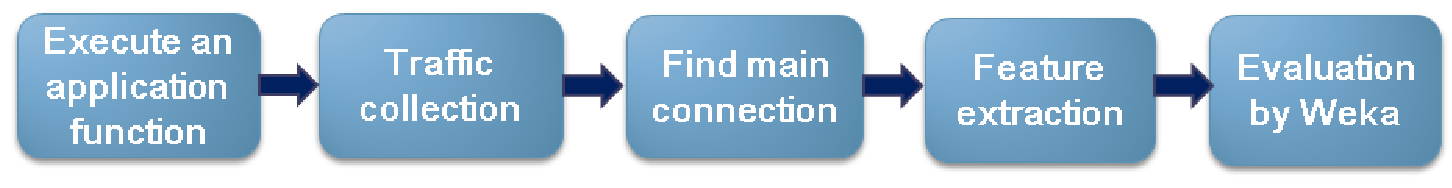
\includegraphics[width=1.0\textwidth]{workflow}
\end{center}
\caption{System workflow of classification.}
\label{Fig.system}
\end{figure}

\section{Traffic Characterization and Classification Evaluation}
\label{sec:evaluation}
In this chapter, we will discuss how to collect the traffic of web applications in detail and present not only the traffic characterization of various web applications, but also the accuracy of their classification.

\subsection{Scenarios of Packet Collection}
\label{sec:scenario}
The network traffic is generated from user interactions on individual applications. We choose the following web applications for analysis: (1) Google docs for the office application, (2) Google map for the map application, (3) Youtube, Tudou, Dailymotion for the video streaming applications, (4) Google drive and Dropbox for the file transfer applications, and (5) Tetris Battle and Dungeon Rampage on Facebook for the game applications. In this work, we repeatedly performed the following actions ten times on either Chrome (version 41.0.2272.89) or Firefox (version 36.0.1) for a period from one to two minutes each time.

The interactions in the office application involve arbitrarily typing characters and changing the colors. The interactions in the map application involve typing an arbitrary location name to be searched in the map, zooming-in and zooming-out the map, and browsing the map. The interactions in the game application involve (1) arbitrarily moving a role and fighting with the other roles in Dungron Rampage and (2) moving and rotating the blocks in Tetris Battle. We also consider the download functions in the video streaming and the file sharing applications. In the former application, we typed an arbitrary video name and moved to a specific time position when watching a video or just silently watched a video until the end. In the latter application, we just downloaded an arbitrary file and waited silently until the completion of the file up/downloading.

\subsection{Traffic Characterization of Web Applications}
\label{sec:characterization}
A typical web session may involve several parallel connections to speed up fetching the requested content, and may also contain irrelevant connections such as those for advertisements. Thus, we manually inspected the content of requests and responses with the developer tools affiliated with the browsers when collecting the related packet traces, and focused only on the connections over which the user interactions are carried. To determine the connections associated with the user interactions, we watched the ongoing connection activities in the developer tool when interacting with a web application, and selected the longest one of these active connections as the main connection. Table~\ref{table:num_connection} presents the average number of connections and the standard deviation in each web application. The values demonstrate that Chrome creates more connections than Firefox on average to transfer the data for the same web applications. 

\begin{table}[h]
\centering
\caption{The average number of connections and the standard deviation (SD) for each web application.}
\label{table:num_connection}
\begin{tabular}{|l|l||l|l||l|l|}
\hline
\multicolumn{2}{|l||}{}                                                                                                                & \multicolumn{2}{l||}{Chrome} & \multicolumn{2}{l|}{Firefox} \\ \hline
Label                                                                     & Web application & Avg.   & SD     & Avg.    & SD   \\ \hline \hline
Document                                                                  & Google doc      & 37.30  & 4.69   & 33.70   & 2.71 \\ \hline
Map                                                                       & Google map      & 27.60  & 2.50   & 19.40   & 1.65 \\ \hline
\multirow{2}{*}{Game}                                                     & \begin{tabular}[c]{@{}l@{}}Dungeon\\ Rampage\end{tabular} 
                  & 125.40 & 10.01  & 108.30  & 7.45 \\ \cline{2-6} 
                                                                     & Tetris Battle   & 218.30 & 14.77  & 174.70  & 8.65 \\ \hline
\multirow{2}{*}{\begin{tabular}[c]{@{}l@{}}File \\ Transfer\end{tabular}} & Google Drive                                              
                  & 37.50  & 3.17   & 31.70   & 0.95 \\ \cline{2-6} 
                                                                        & Dropbox         & 68.00  & 11.26  & 61.30   & 3.30 \\ \hline
\multirow{3}{*}{\begin{tabular}[c]{@{}l@{}}Video \\ Stream\end{tabular}}  & Youtube                                    
                  & 52.3   & 6.02   & 23.70   & 2.63 \\ \cline{2-6} 
                                                                          & Dailymotion     & 380    & 118.08 & 130.50  & 8.67 \\ \cline{2-6} 
                                                                          & Tudou           & 150.80 & 16.60  & 196.30  & 25.19 \\ \hline
\end{tabular}
\end{table}

We analyzed the traffic from the web applications with the developer tools and Wireshark. The traffic characteristics are summarized as follows. In the office application, the characters from user typing are sent in short messages in the same connection from both Chrome and Firefox, and the length of the short massage size for each browser is either 34 bytes or 46 bytes. When we enter the website of the map application, it will display the map of the user's location according to the source IP address. Furthermore, we search a new location, the application will transfer all the data associated with the region to the browser at a time, so no further packets are transferred when we slightly zoom-in and zoom-out the map. When we play Tetris Battle, we find that around 17.28\% of the packets in our each collection contain the TCP PSH flags to ``push'' the packets from the receive buffer to the server application because this game is highly interactive. In the file sharing applications, the client keeps transferring short messages during downloading a file on Google drive. In contrast, there are few messages transferred from the client during file downloading on Dropbox. In video applications except Youtube, the connection that downloads the video clip will be reset when the user changes the time position. 


\subsection{Feature analysis}
\label{sec:feature analysis}
\subsubsection{Message size distribution}
Figure~\ref{Fig.msg_size_distribution} presents the top 10 frequent message sizes from the two browsers in each scenario. The messages are reassembled packet content in the main connections by \texttt{libnids}, and their sizes are ordered by the occurrence frequency. This figure demonstrates that the message sizes in different web applications vary significantly, and the occurrence frequencies of each message size also vary with the applications. The significant variations in different applications imply that the feature of message sizes should be effective for classification. Moreover, the features in the same web applications on different browsers are similar, meaning that the classification is expected to label the applications correctly even though they are running on different browsers.  

\begin{figure}[H]
\centering
\subfloat[Chrome]{
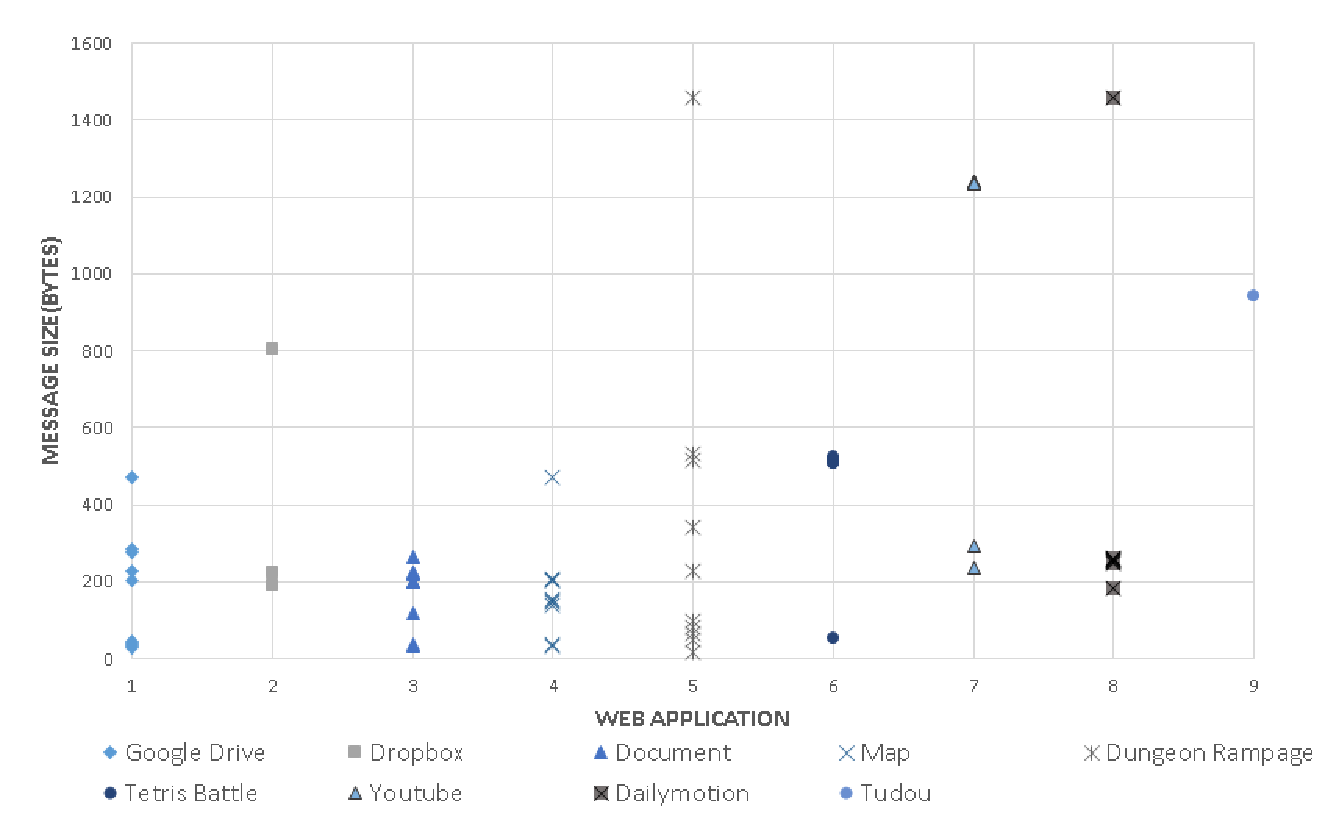
\includegraphics[width=1.0\textwidth]{msg_size_distribution1}
}\\
\subfloat[Firefox]{
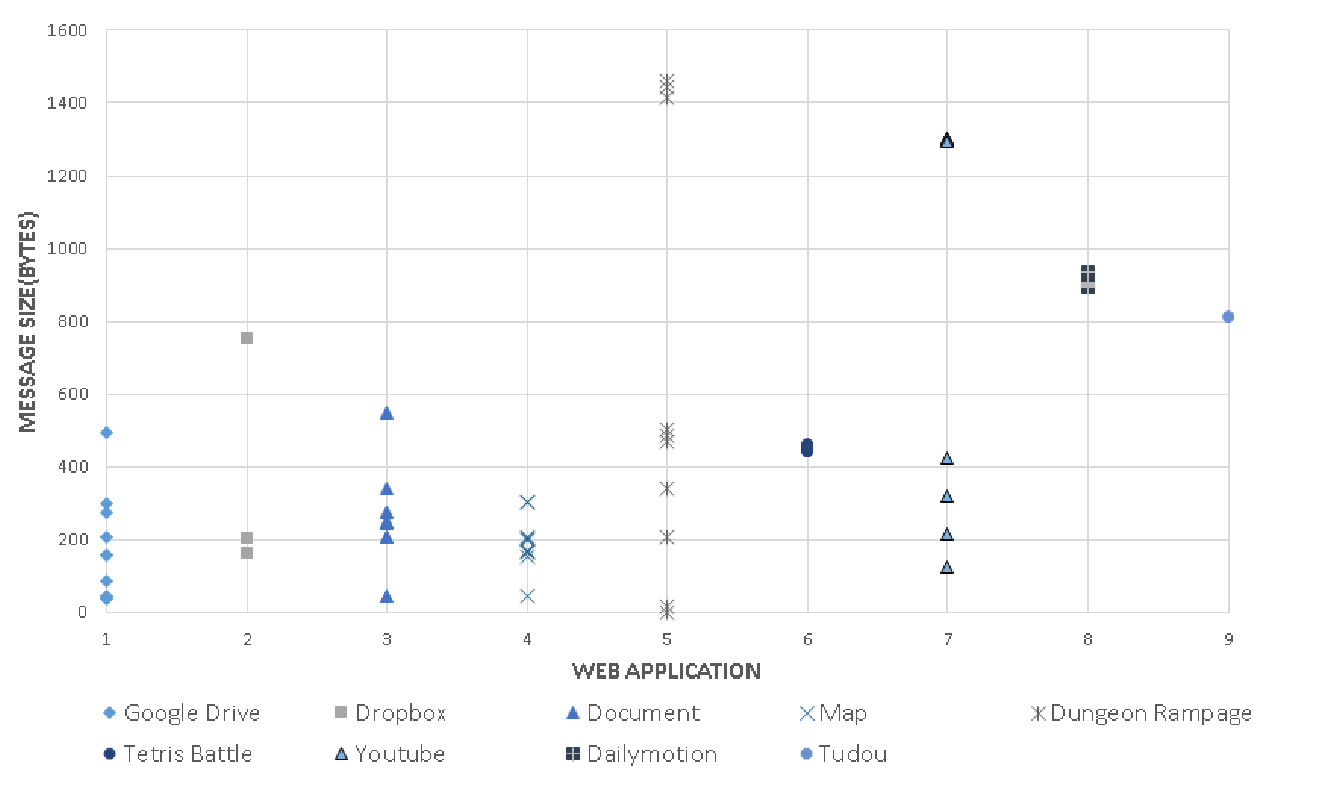
\includegraphics[width=1.0\textwidth]{msg_size_distribution2}
}
\caption{The message size distribution of each web application from two browsers.}
\label{Fig.msg_size_distribution}
\end{figure}

%底下這句的意思是我同樣是在做看影片的動作,但是用不同的平台來觀看會影響feature的結果
Performing the actions on similar web applications will result in different features. For example, the message size distribution of video streaming applications (Youtube, Dailymotion, Tudou) differ obviously according to Figure~\ref{Fig.msg_size_distribution}. However, we do not need to classify individual applications in practice because the management policies (e.g., bandwidth management or QoS) for similar applications are likely to be the same. Thus, we argue that it suffices to classify similar applications into the same category.

Figure~\ref{Fig.setlabel} shows the categorization procedure. We divide the web applications into five categories: file sharing, office, map, game and video streaming. A category consists of one or multiple similar applications. If an application is correctly classified, it is also classified into the correct category. Even though the features are occasionally ambiguous between the applications in the same category (e.g., Dailymotion and Tudou), the applications can be still classified into the category of video streaming applications.   

\begin{figure}[H]
\begin{center} 
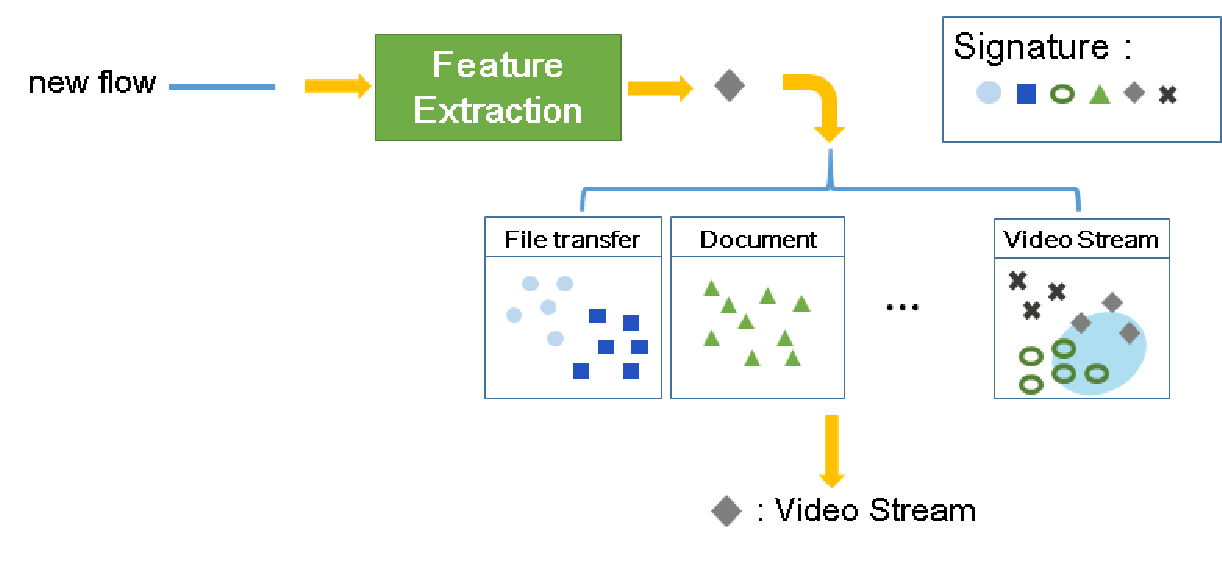
\includegraphics[width=1.0\textwidth]{setlabel}
\end{center}
\caption{Categorization of web applications.}
\label{Fig.setlabel}
\end{figure}


\subsection{Classification results}
\label{sec:result}
After we collect sufficient data from the browsers, we employ Weka to evaluate whether the feature is effective or not. Weka supports a collection of machine learning algorithms for data mining, among which we choose NBtree, Random Forest, J48graft and Naive Bayes to compare the classification accuracy by using different algorithms. We use 10-fold cross-validation to ensure the reliability. When testing the performance, we divide the web applications into two groups, i.e., interaction applications (document, map, game) and file transfer applications (video streaming, file transfer), since we want to compare the result with the previous method, which tests the accuracy of interaction applications and file transfer applications separately. In addition, the possibility of early classification is also evaluated and it will be described in detail on Section 4.4.4.

We choose the previous study to compare with our mechanism. Lin et al. presented the method based on fine-grained classification and used the average and the standard deviation of the request/response lengths as the features for classification. The difference between our targets is that we only want to classify the kinds of web applications; however, they want to distinguish what action a user does. In the work, they subdivide the flows into search keystrokes, editing, action and download. To dislodge the unnecessary message, they artificially input the first request time or the first request bytes. Nevertheless, that method is more suitable for offline analysis. The reason we choose this study as our comparison is that the way of features extraction ,which is independent of the network condition under the application layer, is similar to our mechanism.

\subsubsection{Classification with Similar Interactions in Each Run}
Table~\ref{table:inter_accuracy} shows the classification accuracy of each web application. The accuracy of all classifiers reach 95\% or above with our method, but the values still are slightly lower than previous work. There are some reasons may affect the result. For instance, our targets are different and we do not divide search keystroke messages from the flows we extract, since search packets and interaction packets may be transferred in the same connection. The true-positive rate in Google Map does not achieve 1 is because a few instances of Google Map are misidentified as those of Google document.


\begin{table}[H]
\centering
\caption{True/false positive rates of classifying the interactive connections.}
\label{table:inter_accuracy}
\begin{tabular}{|l|l|l|l|l|l|l|l|l|}
\hline
\multirow{2}{*}{} & \multicolumn{2}{l|}{\begin{tabular}[c]{@{}l@{}}Correctly \\ classified\\      (\%)\end{tabular}} 
				  & \multicolumn{2}{l|}{\begin{tabular}[c]{@{}l@{}}Document\\ \\    TP/FP\end{tabular}}                     
				  & \multicolumn{2}{l|}{\begin{tabular}[c]{@{}l@{}}Map \\     \\    TP/FP\end{tabular}}                   
				  & \multicolumn{2}{l|}{\begin{tabular}[c]{@{}l@{}}Game\\ \\              TP/FP\end{tabular}} \\ \cline{2-9} 
                  & Prior & New &Prior & New & Prior & New & Prior & New \\ \hline \hline
NBtree            & 99.80 & 97.50  & \begin{tabular}[c]{@{}l@{}}0.993/\\ 0.001\end{tabular} & \begin{tabular}[c]{@{}l@{}}1/\\ 0.033\end{tabular}   & \begin{tabular}[c]{@{}l@{}}0.999/\\ 0.005\end{tabular}    & 0.90/0  & 1/0    & 1/0  \\ \hline
RandomForest      & 99.89 & 98.75 & \begin{tabular}[c]{@{}l@{}}1/\\ 0.001\end{tabular}     & \begin{tabular}[c]{@{}l@{}}1/\\ 0.017\end{tabular}   & \begin{tabular}[c]{@{}l@{}}0.999/\\ 0\end{tabular}        & 0.95/0 & 1/0    & 1/0  \\ \hline
J48graft          & 99.28 & 97.50  & \begin{tabular}[c]{@{}l@{}}0.993/\\ 0.004\end{tabular} & \begin{tabular}[c]{@{}l@{}}1/\\ 0.033\end{tabular}   & \begin{tabular}[c]{@{}l@{}}0.996/\\ 0.019\end{tabular}    & 0.90/0  & 0.95/0 & 1/0  \\ \hline
NaiveBayes        & 99.49 & 95.00    & \begin{tabular}[c]{@{}l@{}}0.987/\\ 0\end{tabular}     & \begin{tabular}[c]{@{}l@{}}1/\\ 0.067\end{tabular}   & \begin{tabular}[c]{@{}l@{}}0.996/\\ 0.009\end{tabular}    & 0.80/0  & 1/0    & 1/0  \\ \hline
\multicolumn{9}{r}{Prior: Previous work / New : Our method}\\ 

\end{tabular}
\end{table}


%additional web applications
We also chose three additional web applications to disturb classification: Google sheets (type: document), Bing map (type: map) and Dungeon Blitz (type: game). We followed the scenarios described in Table~\ref{table:scenario_app}, and operated each web applications ten times on either Chrome or Firefox. We gathered the features generated from these additional applications and the original training set to verify the accuracy after the disturbance. The result is showed in Table~\ref{table:add_accuracy} and the accuracy after 10-fold cross-validation can be still up to 97.14\% for NBtree. In this work, we add additional applications only to the group of interaction applications to verify the accuracy because the variation of operations for file transfer applications are usually low.


\begin{table}[H]
\centering
\caption{True/false positive rates of classifying the interactive connections with additional web applications.}
\label{table:add_accuracy}
\begin{tabular}{|l|l|l|l|l|l|l|l|l|}
\hline
\multirow{2}{*}{} & \multicolumn{2}{l|}{\begin{tabular}[c]{@{}l@{}}Correctly\\ classified\\ (\%)\end{tabular}} & \multicolumn{2}{l|}{\begin{tabular}[c]{@{}l@{}}Document\\ \\ TP/FP\end{tabular}}                           & \multicolumn{2}{l|}{\begin{tabular}[c]{@{}l@{}}Map\\ \\ TP/FP\end{tabular}} & \multicolumn{2}{l|}{\begin{tabular}[c]{@{}l@{}}Game\\ \\ TP/FP\end{tabular}} \\ \cline{2-9} 
& Orig. & Add. & Orig. & Add. & Orig. & Add. & Orig. & Add.                                                           \\ \hline
NBtree            & 97.50                                       & 97.14                                       & \begin{tabular}[c]{@{}l@{}}1/\\ 0.033\end{tabular} & \begin{tabular}[c]{@{}l@{}}0.975/\\ 0.03\end{tabular} & 0.90/0        & \begin{tabular}[c]{@{}l@{}}0.925/\\ 0.01\end{tabular}       & 1/0          & 1/0                                                           \\ \hline
RandomRorest      & 98.75                                       & 95.71                                       & \begin{tabular}[c]{@{}l@{}}1/\\ 0.017\end{tabular} & \begin{tabular}[c]{@{}l@{}}0.95/\\ 0.04\end{tabular}  & 0.95/0        & \begin{tabular}[c]{@{}l@{}}0.90/\\ 0.02\end{tabular}        & 1/0          & 1/0                                                           \\ \hline
J48graft          & 97.50                                       & 92.14                                       & \begin{tabular}[c]{@{}l@{}}1/\\ 0.033\end{tabular} & \begin{tabular}[c]{@{}l@{}}0.90/\\ 0.06\end{tabular}  & 0.90/0        & \begin{tabular}[c]{@{}l@{}}0.85/\\ 0.04\end{tabular}        & 1/0          & \begin{tabular}[c]{@{}l@{}}0.983/\\ 0.013\end{tabular}        \\ \hline
NaiveBayes        & 95.00                                       & 95.71                                       & \begin{tabular}[c]{@{}l@{}}1/\\ 0.067\end{tabular} & \begin{tabular}[c]{@{}l@{}}0.975/\\ 0.05\end{tabular} & 0.80/0        & \begin{tabular}[c]{@{}l@{}}0.875/\\ 0.01\end{tabular}       & 1/0          & 1/0                                                           \\ \hline
\multicolumn{9}{r}{Orig.: Original training set / Add.: With additional web applications}\\


\end{tabular}
\end{table}


%file transfer applications
We also differentiate between downloading of video stream and general file transfer. We typed a video name and arbitrarily switched to multiple time positions when watching a video or just silently watched a video until the end on Youtube, Dailymotion and Tudou on the two browsers, but we up/downloaded files by Google drive and Dropbox. In summary, we watched 60 videos and transferred 40 files. After extracting the features, we used 10-fold cross-validation to evaluate the classification. It is presented in Table~\ref{table:file_accuracy} that the classification accuracy can be up to 97\% for all the classifiers, even better than previous work. 

\begin{table}[H]
\centering
\caption{True/false positive rates of classifying downloading connections.}
\label{table:file_accuracy}
\begin{tabular}{|l|l|l|l|l|l|l|}
\hline
\multirow{2}{*}{} & \multicolumn{2}{l|}{\begin{tabular}[c]{@{}l@{}}Correctly \\ classified\\ (\%)\end{tabular}} 
                  & \multicolumn{2}{l|}{\begin{tabular}[c]{@{}l@{}}Video\\ Streaming\\ TP/FP\end{tabular}}                    
                  & \multicolumn{2}{l|}{\begin{tabular}[c]{@{}l@{}}Files\\ Transfer\\ TP/FP\end{tabular}}       \\ \cline{2-7} 
& Prior & New & Prior & New & Prior & New  \\ \hline \hline
NBtree            & 92.72                                            & 97.00                                            & \begin{tabular}[c]{@{}l@{}}0.907/\\ 0\end{tabular} & \begin{tabular}[c]{@{}l@{}}0.967/\\ 0.025\end{tabular} & \begin{tabular}[c]{@{}l@{}}1/\\ 0.093\end{tabular} & \begin{tabular}[c]{@{}l@{}}0.975/\\ 0.033\end{tabular} \\ \hline
RandomForest      & 92.33                                            & 97.00                                            & \begin{tabular}[c]{@{}l@{}}0.902/\\ 0\end{tabular} & \begin{tabular}[c]{@{}l@{}}0.967/\\ 0.025\end{tabular} & \begin{tabular}[c]{@{}l@{}}1/\\ 0.098\end{tabular} & \begin{tabular}[c]{@{}l@{}}0.975/\\ 0.033\end{tabular} \\ \hline
J48graft          & 91.57                                            & 97.00                                            & \begin{tabular}[c]{@{}l@{}}0.893/\\ 0\end{tabular} & \begin{tabular}[c]{@{}l@{}}0.967/\\ 0.025\end{tabular} & \begin{tabular}[c]{@{}l@{}}1/\\ 0.107\end{tabular} & \begin{tabular}[c]{@{}l@{}}0.975/\\ 0.033\end{tabular} \\ \hline
NaiveBayes        & 92.72                                            & 97.00                                            & \begin{tabular}[c]{@{}l@{}}0.907/\\ 0\end{tabular} & \begin{tabular}[c]{@{}l@{}}0.967/\\ 0.025\end{tabular} & \begin{tabular}[c]{@{}l@{}}1/\\ 0.093\end{tabular} & \begin{tabular}[c]{@{}l@{}}0.975/\\ 0.033\end{tabular} \\ \hline
\multicolumn{7}{r}{Prior : Previous work / New : Our method}\\ 

\end{tabular}
\end{table}



\subsubsection{Classification with Diverse Interactions in Each Run}

In this subsection, instead of separating the web applications into interaction function and download function, we classify the traffic into five categories: document, map, game, video stream and file transfer. In the prior study of \cite{TFT14}, the authors evaluated classification separately because the features for interaction function and download function are different in that study, so we also separate the evaluation as well in the last subsection to compare with the prior study fairly. However, we use the same feature, i.e., top-5 most frequent message sizes from the requests, for all the web applications, so we classify all the categories for evaluation in this subsection. We also operated each web application ten times on either Chrome or Firefox, but deliberately performed an extremely different action in the same scenario. For example, we may just continuously type or intermittently edit a document for each time we collected in document function. The classification accuracy after 10-fold cross-validation also can be up to 93.89\% for Random Forest, meaning that the feature is stable and can be used for the classification with high accuracy. 

\begin{table}[H]
\centering
\caption{True/false positive rates of classifying all connections.}
\label{table:all_accuracy}
\begin{tabular}{|l|l|l|l|l|l|l|l|l|l|l|l|l|}
\hline
& \multicolumn{2}{l|}{\begin{tabular}[c]{@{}l@{}}Correctly \\ classified\\  (\%)\end{tabular}} 
& \multicolumn{2}{l|}{\begin{tabular}[c]{@{}l@{}}Document\\ \\ TP/FP\end{tabular}} 
& \multicolumn{2}{l|}{\begin{tabular}[c]{@{}l@{}}Map\\ \\ TP/FP\end{tabular}} 
& \multicolumn{2}{l|}{\begin{tabular}[c]{@{}l@{}}Game\\ \\ TP/FP\end{tabular}} 
& \multicolumn{2}{l|}{\begin{tabular}[c]{@{}l@{}}Video\\  Streaming\\    TP/FP\end{tabular}} 
& \multicolumn{2}{l|}{\begin{tabular}[c]{@{}l@{}}Files\\ Transfer\\ TP/FP\end{tabular}} \\ \hline \hline
NBtree       & \multicolumn{2}{l|}{92.22}                                                                       & \multicolumn{2}{l|}{\begin{tabular}[c]{@{}l@{}}1/\\ 0.05\end{tabular}}                 & \multicolumn{2}{l|}{\begin{tabular}[c]{@{}l@{}}0.80/\\ 0.006\end{tabular}}         & \multicolumn{2}{l|}{\begin{tabular}[c]{@{}l@{}}0.95/\\ 0.007\end{tabular}}   & \multicolumn{2}{l|}{\begin{tabular}[c]{@{}l@{}}0.917/\\ 0\end{tabular}}                  & \multicolumn{2}{l|}{\begin{tabular}[c]{@{}l@{}}0.925/\\ 0.029\end{tabular}}           \\ \hline
RandomForest & \multicolumn{2}{l|}{93.89}                                                                       & \multicolumn{2}{l|}{\begin{tabular}[c]{@{}l@{}}0.90/\\ 0.013\end{tabular}}              & \multicolumn{2}{l|}{\begin{tabular}[c]{@{}l@{}}0.90/\\ 0.019\end{tabular}}         & \multicolumn{2}{l|}{\begin{tabular}[c]{@{}l@{}}0.975/\\ 0.021\end{tabular}}  & \multicolumn{2}{l|}{\begin{tabular}[c]{@{}l@{}}0.933/\\ 0.017\end{tabular}}              & \multicolumn{2}{l|}{\begin{tabular}[c]{@{}l@{}}0.95/\\ 0.007\end{tabular}}            \\ \hline
J48graft     & \multicolumn{2}{l|}{92.22}                                                                       & \multicolumn{2}{l|}{\begin{tabular}[c]{@{}l@{}}0.95/\\ 0.031\end{tabular}}             & \multicolumn{2}{l|}{\begin{tabular}[c]{@{}l@{}}0.80/\\ 0.013\end{tabular}}         & \multicolumn{2}{l|}{\begin{tabular}[c]{@{}l@{}}0.975/\\ 0.021\end{tabular}}  & \multicolumn{2}{l|}{\begin{tabular}[c]{@{}l@{}}0.917/\\ 0.008\end{tabular}}              & \multicolumn{2}{l|}{\begin{tabular}[c]{@{}l@{}}0.925/\\ 0.021\end{tabular}}           \\ \hline
NaiveBayes   & \multicolumn{2}{l|}{92.22}                                                                       & \multicolumn{2}{l|}{\begin{tabular}[c]{@{}l@{}}0.95/\\ 0.025\end{tabular}}             & \multicolumn{2}{l|}{\begin{tabular}[c]{@{}l@{}}0.95/\\ 0.013\end{tabular}}        & \multicolumn{2}{l|}{\begin{tabular}[c]{@{}l@{}}0.95/\\ 0.029\end{tabular}}   & \multicolumn{2}{l|}{\begin{tabular}[c]{@{}l@{}}0.917/\\ 0.017\end{tabular}}              & \multicolumn{2}{l|}{\begin{tabular}[c]{@{}l@{}}0.875/\\ 0.014\end{tabular}}           \\ \hline
\end{tabular}
\end{table}

\subsubsection{Classification with Interactions from Multiple Users}

To ensure the accuracy does not too depend on specific users, we invited eight users to generate the traffic for the classification. In this subsection, we compare only interactive functions because the their actions are more diverse than download functions. The users were asked to perform similar actions to those from a single user and repeated three times for each web applications on Chrome and Firefox. The total number of packet traces is 192: 48 for Google document, 48 for Google map, 48 for Dungeon Rampage and 48 for Tetris Battle.

Table~\ref{table:multi_accuracy} shows the accuracy for each algorithm. We also used 10-fold cross-validation for this classification. The accuracy of our method for Naive Bayes is even higher than the results in Section 4.4, and can be up to 97.92\% with random forest. Compared the result with the training set shown in last subsection, the accuracy is degraded just slightly, meaning that the feature is stable. 

\begin{table}[H]
\centering
\caption{True/false positive rates of classifying the interactive connections for multiple users.}
\label{table:multi_accuracy}
\begin{tabular}{|l|l|l|l|l|l|l|l|l|}
\hline
\multirow{2}{*}{} & \multicolumn{2}{l|}{\begin{tabular}[c]{@{}l@{}}Correctly \\ classified\\      (\%)\end{tabular}} 
				  & \multicolumn{2}{l|}{\begin{tabular}[c]{@{}l@{}}Document\\ \\    TP/FP\end{tabular}}                     
				  & \multicolumn{2}{l|}{\begin{tabular}[c]{@{}l@{}}Map \\     \\    TP/FP\end{tabular}}                   
				  & \multicolumn{2}{l|}{\begin{tabular}[c]{@{}l@{}}Game\\ \\              TP/FP\end{tabular}} \\ \cline{2-9} 
                  & Prior & New & Prior & New & Prior & New & Prior & New \\ \hline \hline

NBtree            & 96.63                                        & 96.35                                        & \begin{tabular}[c]{@{}l@{}}0.939/\\ 0.025\end{tabular} & \begin{tabular}[c]{@{}l@{}}0.938/\\ 0.028\end{tabular} & \begin{tabular}[c]{@{}l@{}}0.971/\\ 0.044\end{tabular} & \begin{tabular}[c]{@{}l@{}}0.938/\\ 0.021\end{tabular} & \begin{tabular}[c]{@{}l@{}}0.993/\\ 0\end{tabular}     & 0.99/0                                                 \\ \hline
RandomForest     & 98.28                                        & 97.92                                        & \begin{tabular}[c]{@{}l@{}}0.954/\\ 0.009\end{tabular} & \begin{tabular}[c]{@{}l@{}}1/\\ 0.007\end{tabular}     & \begin{tabular}[c]{@{}l@{}}0.99/\\ 0.032\end{tabular}  & \begin{tabular}[c]{@{}l@{}}0.979/\\ 0.014\end{tabular} & 1/0                                                    & \begin{tabular}[c]{@{}l@{}}0.969/\\ 0.01\end{tabular}  \\ \hline
J48graft         & 97.65                                        & 93.75                                        & \begin{tabular}[c]{@{}l@{}}0.939/\\ 0.011\end{tabular} & \begin{tabular}[c]{@{}l@{}}0.917/\\ 0.035\end{tabular} & \begin{tabular}[c]{@{}l@{}}0.986/\\ 0.044\end{tabular} & \begin{tabular}[c]{@{}l@{}}0.917/\\ 0.035\end{tabular} & \begin{tabular}[c]{@{}l@{}}0.993/\\ 0.001\end{tabular} & \begin{tabular}[c]{@{}l@{}}0.958/\\ 0.021\end{tabular} \\ \hline
NaiveBayes       & 95.74                                        & 95.83                                        & \begin{tabular}[c]{@{}l@{}}0.87/\\ 0.017\end{tabular}  & \begin{tabular}[c]{@{}l@{}}0.938/\\ 0.028\end{tabular} & \begin{tabular}[c]{@{}l@{}}0.98/\\ 0.091\end{tabular}  & \begin{tabular}[c]{@{}l@{}}0.938/\\ 0.028\end{tabular} & \begin{tabular}[c]{@{}l@{}}1/\\ 0.001\end{tabular}     & \begin{tabular}[c]{@{}l@{}}0.979/\\ 0\end{tabular}     \\ \hline

\multicolumn{9}{r}{Pre: Previous work / New : Our method}\\ 

\end{tabular}
\end{table}


\subsubsection{Early Classification}
\label{sec:early}
The classification method in this work can be applied to manage various web applications, even though the web traffic is encrypted. The specifics of classification may vary in practice, depending on the purpose of management. If the purpose is accounting the usage of web applications in a network, it would suffice to classify the web applications offline based on the features from \emph{the entire packet traces} that have been observed. However, if the purpose is access control, classification after extracting the features from the entire packet traces will be too late to block the traffic in time. Thus, we also evaluate the effectiveness of early classification with the features from the partial messages in the beginning of the connections. In early classification, a connection can be blocked as soon as the web application is recognized based on the features from the partial messages. 

The packet traces for evaluating early classification are same as those described in the last subsection. We extracted the first $k$ messages from each main connection ($k=15, 20, 25, 30, 50, 100$) and used the size distribution of only these messages for the evaluation. Like the features from the entire packet traces, we also extracted the top five frequent message sizes in terms of occurrence frequency.  

The previous analysis show that the true-positive rate of almost all kinds of functions are at least up to 0.90; however, the true-positive rate for the map application is decreased to 0.80 because its features are not so stable as others. We choose Dungeon Rampage on Chrome as example for stable one shown as Figure~\ref{Fig.set_size_dr} and Google map on Chrome as example for unstable one shown as Figure~\ref{Fig.set_size_map}. The line chart is created by entire messages within a main connection and the scatter chart is created by the first $k$ messages in each figure.

\begin{figure}[H]
\begin{center} 
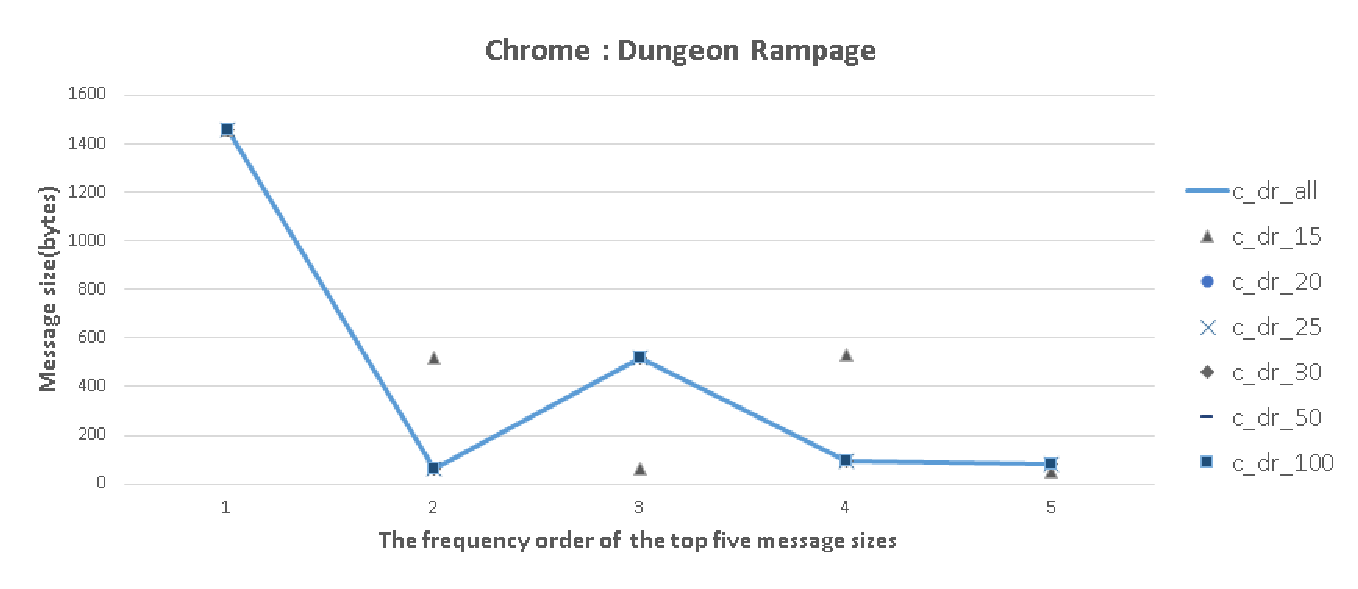
\includegraphics[width=1.1\textwidth]{early_dr}
\end{center}
\caption{The message size distribution for Dungeon Rampage.}
\label{Fig.set_size_dr}
\end{figure}

Figure~\ref{Fig.set_size_dr} depicts that the scatter charts are similar with the trend of line chart when we extract more than the first 20 messages. Figure~\ref{Fig.set_size_map} depicts that the scatter charts are almost similar with the trend of line chart when we extract more than the first 30 messages. So we finally extracted the first 30 messages from each web applications as our feature for early classification. The classification accuracy after 10-fold cross-validation can be at least 86.67\% and even can be up to 93.89\% for Random Forest.


\begin{figure}[H]
\begin{center} 
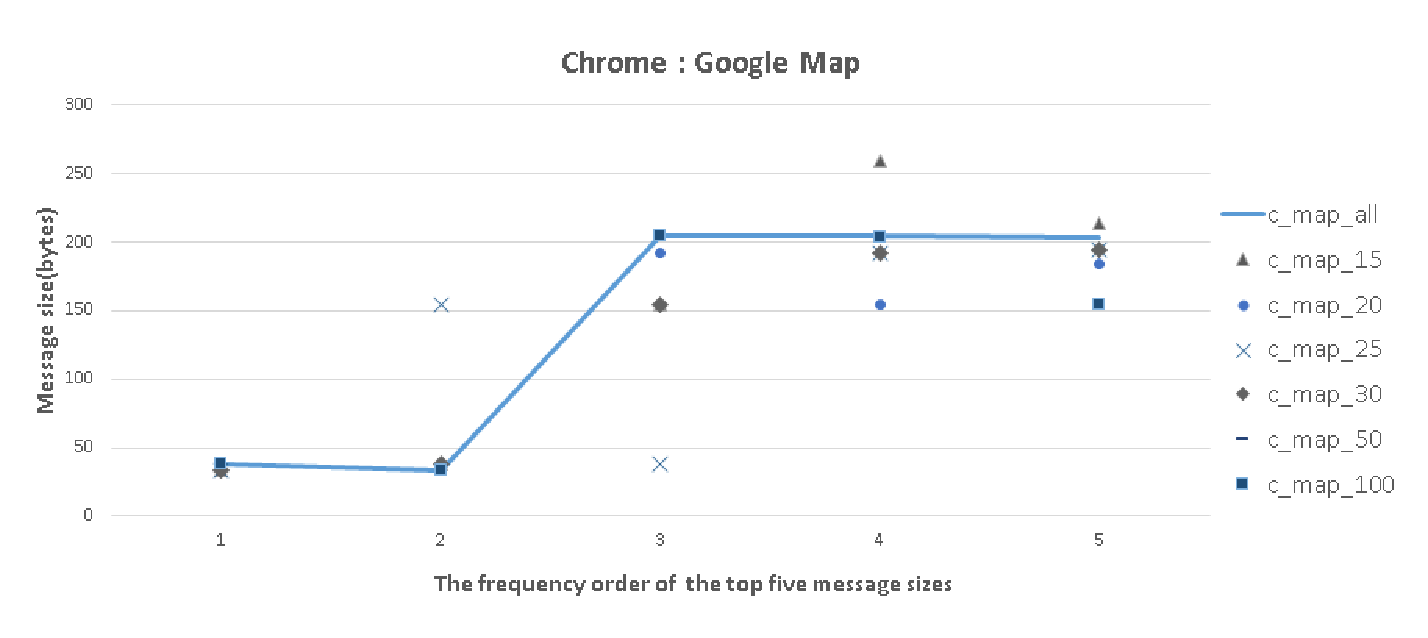
\includegraphics[width=1.1\textwidth]{early_map}
\end{center}
\caption{The message size distribution for Google map.}
\label{Fig.set_size_map}
\end{figure}

\begin{table}[H]
\centering
\caption{Early classification true/false positive rate in all connections.}
\label{table:early_accuracy}
\begin{tabular}{|l|l|l|l|l|l|l|}
\hline
& \begin{tabular}[c]{@{}l@{}}Correctly \\ classified\\ (\%)\end{tabular} 
& \begin{tabular}[c]{@{}l@{}}Document\\ \\ TP/FP\end{tabular} 
& \begin{tabular}[c]{@{}l@{}}Map \\ \\ TP/FP\end{tabular} 
& \begin{tabular}[c]{@{}l@{}}Game\\ \\ TP/FP\end{tabular} 
& \begin{tabular}[c]{@{}l@{}}Video\\ Stream\\ TP/FP\end{tabular} 
& \begin{tabular}[c]{@{}l@{}}File\\ Transfer\\ TP/FP\end{tabular} \\ \hline \hline
NBtree       & 86.67         & \begin{tabular}[c]{@{}l@{}}0.70/\\ 0.038\end{tabular}  & \begin{tabular}[c]{@{}l@{}}0.95/\\ 0.019\end{tabular}         & \begin{tabular}[c]{@{}l@{}}0.925/\\ 0.007\end{tabular}           & \begin{tabular}[c]{@{}l@{}}0.933/\\ 0.025\end{tabular} & \begin{tabular}[c]{@{}l@{}}0.75/\\ 0.079\end{tabular}           \\ \hline
RandomForest & 93.89         & \begin{tabular}[c]{@{}l@{}}0.85/\\ 0.013\end{tabular}  & 1/0                                                           & \begin{tabular}[c]{@{}l@{}}1/\\ 0.014\end{tabular}           & \begin{tabular}[c]{@{}l@{}}0.933/\\ 0.017\end{tabular} & \begin{tabular}[c]{@{}l@{}}0.90/\\ 0.036\end{tabular}           \\ \hline
J48graft     & 88.33         & \begin{tabular}[c]{@{}l@{}}0.85/\\ 0.019\end{tabular}  & \begin{tabular}[c]{@{}l@{}}1/\\ 0.019\end{tabular}            & \begin{tabular}[c]{@{}l@{}}0.95/\\ 0.029\end{tabular}           & \begin{tabular}[c]{@{}l@{}}0.85/\\ 0.042\end{tabular}  & \begin{tabular}[c]{@{}l@{}}0.825/\\ 0.043\end{tabular}          \\ \hline
NaïveBayes   & 87.22         & \begin{tabular}[c]{@{}l@{}}0.85/\\ 0.063\end{tabular}  & \begin{tabular}[c]{@{}l@{}}0.95\\ /0.013\end{tabular}         & \begin{tabular}[c]{@{}l@{}}0.925/\\ 0.021\end{tabular}           & \begin{tabular}[c]{@{}l@{}}0.95/\\ 0.017\end{tabular}  & \begin{tabular}[c]{@{}l@{}}0.675/\\ 0.043\end{tabular}          \\ \hline
\end{tabular}
\end{table}

\subsection{Practice and Limitation}
\label{sec:app_limit}

Even though the classification accuracy is high for extracted packet traces from real user interactions with web applications, there are still some issues that should be addressed to deploy this classification in practice.

First, although one IP address may be associated with more than one web application, as we demonstrated earlier in this work, we can still record the mapping between the IP addresses and their associated applications from earlier classification in a list to speed up classification. Since the mapping may be one-to-many, if a remote IP address can be found in the list and it is mapped to only one application, we can leverage the result of earlier classification to label the traffic to that application directly; otherwise, we can follow the procedure described in Chapter 3 to classify the web application. The result from earlier classification can at least help reduce the scope of possible labels.

Second, the traffic for each packet trace is just generated from a specific web application in this work, but in reality, we will need to analyze multiple applications at the same time and extracting the main connection is a problem. To solve this issue, we will observe the traffic density and quantity of each IP address during a period time and if the values both reach the thresholds, we will extract it as the main connection for classification. After classification, if the device that employs the design determines to block the main connection, the connections having the same pair of source/destination IP addresses as the main connection and happening around it will be blocked as well. Furthermore, users may use a web application not in the training set. Thus, after traffic classification, we will have to compute the distance between the feature vectors of the analyzed traffic and the application(s) that the analyzed traffic is supposed to be. If the distance is too long, than the analyzed traffic will be labeled as unknown.


Third, if the main connection is identified after the web application has been executed for a period of time, it may be too late to block an application for access control since the function is likely to have already completed its execution when the flows are collected and analyzed. The early classification described in Section~\ref{sec:early} can address this issue. Moreover, the accuracy may be decreased if the execution time of an web application function is too short to extract meaningful feature.

\section{Conclusion}
\label{sec:conclusion}
In this work, we classify the web application and focus on the five categories of web applications: office application, map application, game application, video streaming application and file sharing application. The statistical features are extracted from application-level and need not to analyze the packet payloads, so we do not have to concern about the network condition and the encryption issue. All of the data sets are generated artificially, so the condition is close to reality. This work uses Weka and 10-fold cross-validation for evaluating the classification accuracy.

The experimental results demonstrate that the accuracy can be as high as 98.75\% and the false-positive rate is no more than 0.017 using random forest for the interaction functions. For the download functions, the accuracy can be up to 97.00\% and the false-positive rate can be 0.025 for each algorithm. For the five functions, the accuracy can be up to 93.89\% and the false-positive rate can be 0.007 using random forest. For the early classification, the accuracy can be up to 93.89\% and the false-positive rate is no more than 0.036 using random forest. Finally, the results show that the feature can effectively classify traffic of various web applications, and even in early classification. 

%\section*{Acknowledgment}
%
%This work was supported by National Science Council (NSC) Project 98-2218-E-194-009.

%% The Appendices part is started with the command \appendix;
%% appendix sections are then done as normal sections
%% \appendix

%% \label{}

%% References
%%
%% Following citation commands can be used in the body text:
%%
%%  \citet{key}  ==>>  Jones et al. (1990)
%%  \citep{key}  ==>>  (Jones et al., 1990)
%%
%% Multiple citations as normal:
%% \citep{key1,key2}         ==>> (Jones et al., 1990; Smith, 1989)
%%                            or  (Jones et al., 1990, 1991)
%%                            or  (Jones et al., 1990a,b)
%% \cite{key} is the equivalent of \citet{key} in author-year mode
%%
%% Full author lists may be forced with \citept* or \citepp*, e.g.
%%   \citep*{key}            ==>> (Jones, Baker, and Williams, 1990)
%%
%% Optional notes as:
%%   \citep[chap. 2]{key}    ==>> (Jones et al., 1990, chap. 2)
%%   \citep[e.g.,][]{key}    ==>> (e.g., Jones et al., 1990)
%%   \citep[see][pg. 34]{key}==>> (see Jones et al., 1990, pg. 34)
%%  (Note: in standard LaTeX, only one note is allowed, after the ref.
%%   Here, one note is like the standard, two make pre- and post-notes.)
%%
%%   \citealt{key}          ==>> Jones et al. 1990
%%   \citealt*{key}         ==>> Jones, Baker, and Williams 1990
%%   \citealp{key}          ==>> Jones et al., 1990
%%   \citealp*{key}         ==>> Jones, Baker, and Williams, 1990
%%
%% Additional citation possibilities
%%   \citeauthor{key}       ==>> Jones et al.
%%   \citeauthor*{key}      ==>> Jones, Baker, and Williams
%%   \citeyear{key}         ==>> 1990
%%   \citeyearpar{key}      ==>> (1990)
%%   \citetext{priv. comm.} ==>> (priv. comm.)
%%   \citenum{key}          ==>> 11 [non-superscripted]
%% Note: full author lists depends on whether the bib style supports them;
%%       if not, the abbreviated list is printed even when full requested.
%%
%% For names like della Robbia at the start of a sentence, use
%%   \citet{dRob98}         ==>> Della Robbia (1998)
%%   \citep{dRob98}         ==>> (Della Robbia, 1998)
%%   \citeauthor{dRob98}    ==>> Della Robbia


%% References with bibTeX database:
\bibliographystyle{elsarticle-num}
\bibliography{tc-jnca}

%% Authors are advised to submit their bibtex database files. They are
%% requested to list a bibtex style file in the manuscript if they do
%% not want to use model4-names.bst.

%% References without bibTeX database:

% \begin{thebibliography}{00}

%% \bibitem must have one of the following forms:
%%   \bibitem[Jones et al.(1990)]{key}...
%%   \bibitem[Jones et al.(1990)Jones, Baker, and Williams]{key}...
%%   \bibitem[Jones et al., 1990]{key}...
%%   \bibitem[\protect\citeauthoryear{Jones, Baker, and Williams}{Jones
%%       et al.}{1990}]{key}...
%%   \bibitem[\protect\citeauthoryear{Jones et al.}{1990}]{key}...
%%   \bibitem[\protect\astroncite{Jones et al.}{1990}]{key}...
%%   \bibitem[\protect\citename{Jones et al., }1990]{key}...
%%   \harvarditem[Jones et al.]{Jones, Baker, and Williams}{1990}{key}...
%%

% \bibitem[ ()]{}

% \end{thebibliography}

\end{document}

%%
%% End of file `elsarticle-template-4-harv.tex'.
